\chapter{Experimental results}

In this chapter, we present experimental results of our tool on several code-breaking games.
We compare running times of the tool on various tasks with different SAT solvers and
  evaluate presented one-step look-ahead strategies.

In the tables below, MM($n$,$m$) refers to Mastermind with $n$ pegs and $m$ colours,
CC($n$) refers to the counterfeit coin problem with $n$ coins,
BG($n$,$m$) refers to Bags of gold problem with $n$ bags and balance scale capacity $m$ and
SM($n$,$m$) refers to the Mastermind variant with black markers only, i.e.
  for each guess, the codebreaker gets the number of positions at which the code
  and the guess match.

\section{Performance}

All experiments have been run on Intel Core i7-3770 3.40GHz and COBRA was
compiled with \texttt{gcc} 4.8.2.
The symmetry breaking engine has been turned off for this section,
  so that the differences among SAT solvers become more apparent.

The numbers in the following tables are running times in seconds with
  respective SAT solvers.
The last column (``\# calls'') states the total number of calls to
  the SAT solver during the task.
Model counting and counting the number of fixed variables is considered one call.

\autoref{tbl:exp-sat-wellformed} lists running times of the well-formed check
  of several code-breaking games.
Naturally, proper SAT solvers are orders of magnitude faster than simple solver
as well-formed check is based on verification of unsatisfiability of
  a (relatively) large formula.

\begin{table}[h]
\begin{center}
\begin{tabular}{|l|c|c|c|c|} \hline
Game & Simple & Minisat & Picosat  & \# calls \\ \hline
MM(4,6) & 174 & \textbf{2.7} & 3.2 & 1,296 \\
MM(5,4) & 217 & \textbf{14.3} & 34.8 & 1,024 \\
BG(12,12) & 3,539 &  \textbf{0.5} & 1.1 & 271 \\\hline
\end{tabular}
\caption{Running times (in seconds) of the well-formed check.}
\label{tbl:exp-sat-wellformed}
\end{center}
\end{table}

The first two lines of \autoref{tbl:exp-sat-sim} shows execution times of the
  first experiment selection in Mastermind with $4$ pegs and $6$ colours.
The last two lines of the table list running times of the simulation of
  respective strategies on EDEE code.

As can be seen from the numbers, evaluation of ``parts'' strategy is slightly
  faster with Minisat than with simple solver.
However, since our model counting algorithm implemented on top of Minisat and Picosat
  is na\"ive and unoptimized, ``max-models'' strategy evaluation is significantly faster
  with simple solver.

\begin{table}[h]
\begin{center}
\begin{tabular}{|l|c|c|c|c|} \hline
Task & Simple & Minisat & Picosat & \# calls \\ \hline
Select first exp. (parts) & 3.9 & \textbf{2.6} & 523 & 17,108 \\
Select first exp. (max-models) & \textbf{9.3} & 45.3 & $>$ 5,000 & 3,145 \\
Simulate (parts on EDEE) & 10.5 & \textbf{7.9} & 749 & 92,644 \\
Simulate (max-models on EDEE) & \textbf{15.1} & 32.3 & 3,024 & 31,061 \\\hline
\end{tabular}
\caption{Running times (in seconds) of simulation and strategy evaluation on MM(4,6).}
\label{tbl:exp-sat-sim}
\end{center}
\end{table}

\autoref{tbl:exp-sat-analyse}
  shows running times of strategy analysis.
A clear winner in this case is the simple solver based on
  model enumeration,
  which is not unexpected.
On lower levels of the backtracking algorithm,
  the analysed formulas has only very few models and the
  overhead with calling a proper SAT solver is greater
  than the na\"ive approach of a simple solver.

The results also show that model counting is harder than satisfiability questions.
The difference is not that significant for simple solver
 but, as we have already mentioned, our model counting algorithm is much slower.
That is the reason why the analysis of ``max-models'' strategy takes Minisat and Picosat
  much more time than analysis of ``parts'' strategy.

To summarize the results of this section,
Picosat turned out to be very slow on instances of this size. Minisat proved
useful for strategy evaluation in the first rounds, when the number of possible
models of the formula is relatively large.
Simple solver is a clear winner for strategy analysis.

A question arises whether we can benefit from a hybrid approach of
  using a SAT solver in the first steps and
  switching to the simple solver when the number of possibilities shrinks.
This was, however, beyond the scope of this thesis.

\begin{table}
\begin{center}
\begin{tabular}{|l|l|c|c|c|c|} \hline
Game & Strategy& Simple & Minisat & Picosat & \# calls \\ \hline
MM(3,4) & parts & 0.1 & 0.4 & 13.5 & 13,769 \\
MM(3,4) & max-models & 0.1 & 2.1 & 179 & 9,349 \\
MM(3,4) & exp-fixed & 0.3 & 17.4 & 1,974 & 15,002 \\
MM(4,4) & parts & 6.9 & 237 & $>$ 5,000 & 260,144 \\
MM(4,4) & max-models & 5.0 & 1,126 & $>$ 5,000 & 188,828 \\
MM(4,4) & exp-fixed & 24 & $>$ 5,000 & $>$ 5,000 & 329,820 \\
CC(20) & parts & 0.1 & 0.3 & 12.8 & 7,718 \\
CC(20) & max-models & 0.2 & 28 & 3,161 & 12,117 \\
CC(20) & exp-fixed & 0.3 & 73 & $>$ 5,000 & 14,273 \\\hline
% Analyse parts & CC(30) &  6.87 & 237 & ? & 260,144 \\
% Analyse parts & CC(30) &  0.08 & 0.34 & 13.5 & 13,769 \\
% Analyse max-models & CC(30) & ? & ? & ? & ? \\
% Analyse max-models & CC() & ? & ? & ? & ? \\
\end{tabular}
\caption{Running times (in seconds) of strategy analysis.}
\label{tbl:exp-sat-analyse}
\end{center}
\end{table}


\section{One-step look-ahead strategies}

In this section, we compare performance of one-step look-ahead strategies
defined in \autoref{sec:oslas} on the counterfeit coin problem,
Mastermind, and Mastermind with black markers only.

\subsection{The counterfeit coin problem}

The average-case number of experiments performed by one-step look-ahead
  strategies in the counterfeit coin problem
  for the number of coins from 3 to 40 is shown in \autoref{fig:exp-cc}.

Notice that larger number of coins does not necessarily mean that
  identifying the counterfeit coin is more difficult.
For example, the ``max-models'' strategy needs
  3.44 experiments on average to identify the counterfeit coin
  among 16 coins but only 3.41 if the number of coins is 17.
That is because the additional coin changes
  the numbers of models of some outcomes,
  which may lead to better experiment selection.

Interestingly, ``exp-fixed'' strategy outperforms all others
  on 20, 21, 23, 25 and 27 coins, while it seems to be
  generally worse.
Strategies ``parts'' and ``min-fixed'' are clearly unsuitable for
  a problem of this kind.

\begin{figure}[h]
\begin{center}
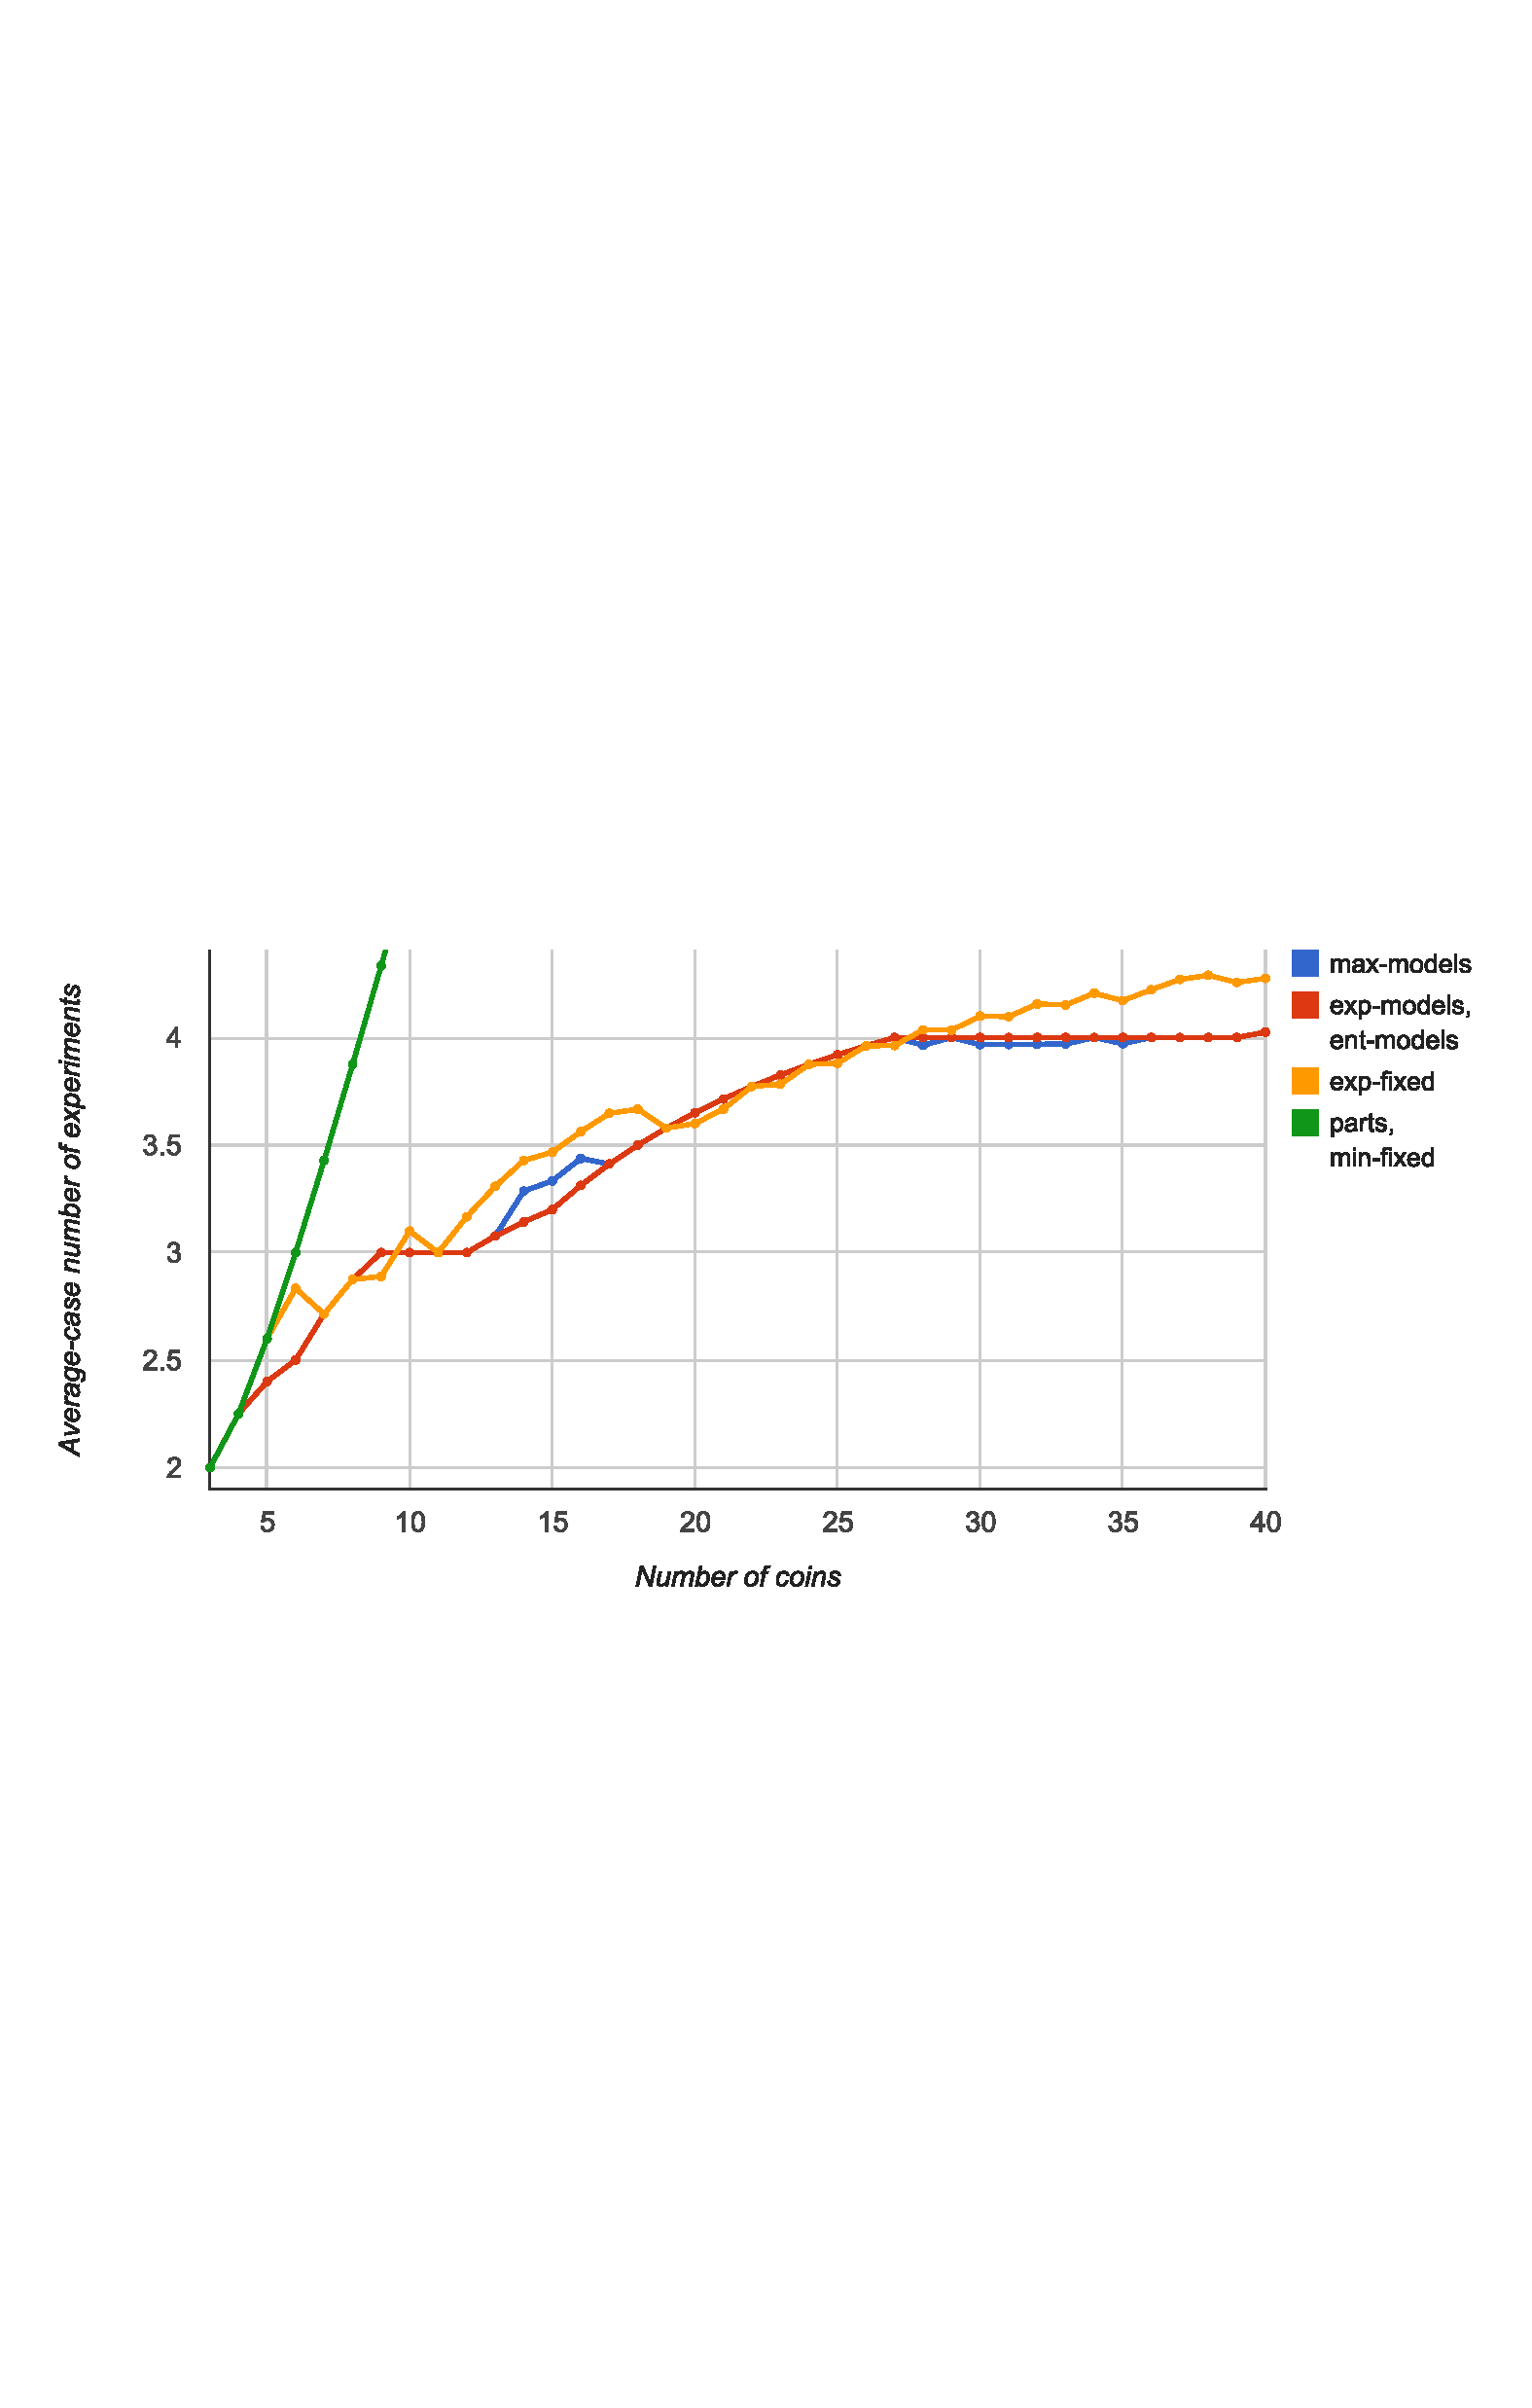
\includegraphics[width=\textwidth]{pictures/graph-cc.pdf}
\caption{Average-case number of experiments in the counterfeit coin problem.}
\label{fig:exp-cc}
\end{center}
\end{figure}

\subsection{Mastermind}

Results for Mastermind are shown in \autoref{tbl:exp-mm},
  rounded to three decimal places.
A clear winner in the average case is ``parts'' strategy,
  closely followed by ``max-models''.

In the worst case, ``max-models'' outperforms other
  strategies in all cases except MM(3,2).
This case was already mentioned in \TODO{..};
  the strategy needs four experiments due to an ``unlucky''
  choice of the first experiments.

Again, notice that larger size of the problem does not necessarily mean that
  revealing the secret is more difficult,
  as can be seen on the values for MM(5,2) and MM(5,3).

\begin{table}[h]
\begin{center}
\begin{tabular}{|c|c|c|c|c|c|c|c|c|c|c|c|c|}\hline
Game & \multicolumn{2}{c|}{max-mod} & \multicolumn{2}{c|}{parts}
& \multicolumn{2}{c|}{exp-mod} & \multicolumn{2}{c|}{ent-mod}
& \multicolumn{2}{c|}{min-fix} & \multicolumn{2}{c|}{exp-fix}\\ \hline
MM(2,3) & 2.667 & 4 & 2.333 & 3 & 2.444 & 3 & 2.444 & 3 & 2.667 & 4 & 2.444 & 3 \\
MM(2,6) & 3.667 & 5 & 3.667 & 5 & 3.861 & 5 & 3.861 & 5 & 4.611 & 7 & 4.167 & 6 \\\hline
MM(3,2) & 2.625 & 4 & 2.250 & 3 & 2.250 & 3 & 2.250 & 3 & 2.625 & 4 & 2.25 &  3 \\
MM(3,6) & 4.046 & 5 & 3.977 & 5 & 4.227 & 5 & 4.218 & 5 & 5.259 & 8 & 4.546 & 6 \\
MM(3,8) & 4.787 & 6 & 4.701 & 6 & 4.879 & 6 & 4.844 & 6 & 6.688 & 10 & 5.631 & 8 \\\hline
MM(4,2) & 2.750 & 4 & 2.750 & 4 & 3.063 & 4 & 3.063 & 4 & 3.250 & 5 & 3.063 & 4 \\
MM(4,6) & 4.476 & 5 & 4.374 & 6 & 4.626 & 6 & 4.643 & 6 & 5.765 & 9 & 5.231 & 7 \\
MM(4,7) & 4.837 & 6 & 4.743 & 6 & 4.962 & 6 & 4.947 & 6 & 6.476 & 10 & 5.945 & 8 \\
MM(4,8) & 5.183 & 6 & 5.102 & 7 & 5.293 & 7 & 5.272 & 7 & 7.213 & 11 & 6.410 & 9 \\\hline
MM(5,2) & 3.500 & 5 & 3.313 & 5 & 3.938 & 5 & 3.625 & 5 & 3.875 & 6 & 3.781 & 5 \\
MM(5,3) & 3.407 & 4 & 3.379 & 4 & 3.634 & 4 & 3.609 & 4 & 4.444 & 7 & 3.942 & 5 \\
MM(5,4) & 3.991 & 5 & 3.880 & 5 & 4.092 & 5 & 4.083 & 5 & 5.014 & 9 & 4.617 & 6 \\\hline
\end{tabular}
\caption{Average-case and worst-case number of experiments\\
  of one-step look-ahead strategies in Mastermind.}
\label{tbl:exp-mm}
\end{center}
\end{table}


\subsection{Mastermind with black markers only (string matching)}

Mastermind with black markers only is an example of a code-breaking game,
  where ``max-models'' does not perform so well.
Exact values rounded to two decimal points are shown in \autoref{tbl:exp-mmb}.

The best one-step look-ahead startegy for this game is ``ent-models'',
  the strategy based on the entropy of the number of models,
  closely followed by ``parts'' strategy.

\begin{table}[f]
\begin{center}
\begin{small}
\begin{tabular}{|c|c|c|c|c|c|c|c|c|c|c|c|c|}\hline
Game & \multicolumn{2}{c|}{max-mod} & \multicolumn{2}{c|}{parts}
& \multicolumn{2}{c|}{exp-mod} & \multicolumn{2}{c|}{ent-mod}
& \multicolumn{2}{c|}{min-fix} & \multicolumn{2}{c|}{exp-fix}\\ \hline
SM(3,3) & 3.15 &  4 &  2.89 & 4 & 2.89 & 4 & 2.89 & 4 & 3.52 &  4 & 3.52 &  4 \\
SM(3,6) & 6.1 &  8 &  5.58 & 7 & 5.74 & 8 & 5.53 & 7 & 8.3 & 13 &  8.28 &  13 \\
SM(3,12)& 10.76& 14 & 10.28 & 13& 10.5 & 14 & 10.23 & 13 &  17.41 & 31 &  13.3 &  22 \\ \hline
SM(6,3)& 4.94 &  6 &  4.5 & 7 & 4.5 & 6 & 4.47 &  6 & 6.5 & 7 & 6.16 &  7 \\
SM(6,6)& 8.61 & 12 &  8.2 & 12& 7.99 & 11 & 7.93 & 11 &  15.8 &  25 &  15.75 & 25 \\ \hline
\end{tabular}
\end{small}
\caption{Average-case and worst-case number of experiments
  of one-step look-ahead strategies \\ in Mastermind with black markers only.}
\label{tbl:exp-mmb}
\end{center}
\end{table}

